%% part4
\MinParskip{}

\subsection{The Entropy Weight Method (EWM) }
We use the Entropy Weight Method (EWM) to get the weight of indicators. The Entropy Weight Method is an object weighting method, which uses the information entropy idea for reference. It is used to determine the relative weights of different criteria in a decision-making process. It determines the weight of the indicators by calculating the information entropy of the index, according to the impact of the relative change of the index on the overall system.

In other words, the weight of each indicator is given according to the difference degree of the indicator value, and the corresponding weight of each indicator is obtained. The indicator with relatively large change degree has larger weight. 

The greater the entropy, the more chaotic the system is, the less information it carries and the less weight it has. Otherwise, the higher the entropy, the more orderly the system is, the more information it carries, and the greater the weight is.

The first step of the Entropy Weight Method is the standardization of measured values. The standardized value of the jth index in the ith sample is denoted as $p_{ij}$, and its calculation method is as follows:$$p_{ij}=\frac{a_{ij}}{\sum_{i=1}^na_{ij}},i=1,2\cdots,,9,j=1,2,\cdots,9$$

Secondly, in the EWM, the entropy value $e_i$ of the jth index is defined as:$$e_j=-\frac{1}{ln(9)}\sum_{i=1}^np_{ij}ln(p_{ij}),j=1,2,\cdots,9$$

The range of entropy value $e_j$ is [0, 1]. The larger the $e_j$ is, the greater the differentiation degree of index j is, and more information can be derived. Hence, higher weight should be given to the index. 

Finally, the calculation method of weight is:$$w_j=\frac{1-e_j}{\sum_{j=1}^me_j},j=1,2,\cdots,9$$

Through the three steps, we can easily get the weight of each indicator.


\subsection{The TOPSIS Method}

The Technique for Order of Preference by Similarity to Ideal Solution (TOPSIS) is a multi-criteria decision-making method that is used to determine the best option from a set of alternatives based on multiple criteria. 

First of all, we use Min-Max normalization to process the data.

For the benefit-attributed data,
$$b_{ij}=\frac{a_{ij}-a_j^{min}}{a_j^{max}-a_j^{min}}$$

And for the cost-attributed data,
$$b_{ij}=\frac{a_{j}^{max}-a_{ij}}{a_j^{max}-a_j^{min}}$$

All these data from the normalized matrix $B$. We then multiply each value in a column with the corresponding weight given, and get weighted-normalised decision matrix, which $$C=W*B$$

Secondly, calculating the ideal best and the ideal worst. Now we need to calculate Euclidean distance for elements in all rows from the ideal best and the ideal worst. Here, $s_i^*$ is the best distance calculated on the i-th row, where $b_{ij}$ is element value and $C_i^{*}$ is the ideal best for that column. Similarly, we can find $s_i^0$, which is the worst distance calculated on the i-th row.

\begin{table}[H] \centering
    \caption{Weights of the Indicators Calculated from TOPSIS}
    \begin{tabular}{ccl}
        \toprule
        Indicators & Weights\\ \hline
        All industry total & 0.36639\\
        All tertiary industry percentage & 0.01866\\
        Population Density & 0.43171\\
        Limiting Magnitude & 0.01781\\
        Last Bus Time & 0.06481\\
        Power Consumption per Capita per Month & 0.00091\\
        Annual Precipitation(in millimetre) & 0.08705\\
        Work hours per Week & 0.00003\\
        Nightlife index & 0.01263\\
        \bottomrule
    \end{tabular}
\end{table}

Finally, calculate the TOPSIS Score and Ranking. Now we have distance positive and distance negative, calculate the Topsis score for each row based on them in the end.

\subsection{Application of the Model on the Four Locations}


\subsubsection{A Protected Land Location: Wyoming}
\begin{figure}[H]\centering
    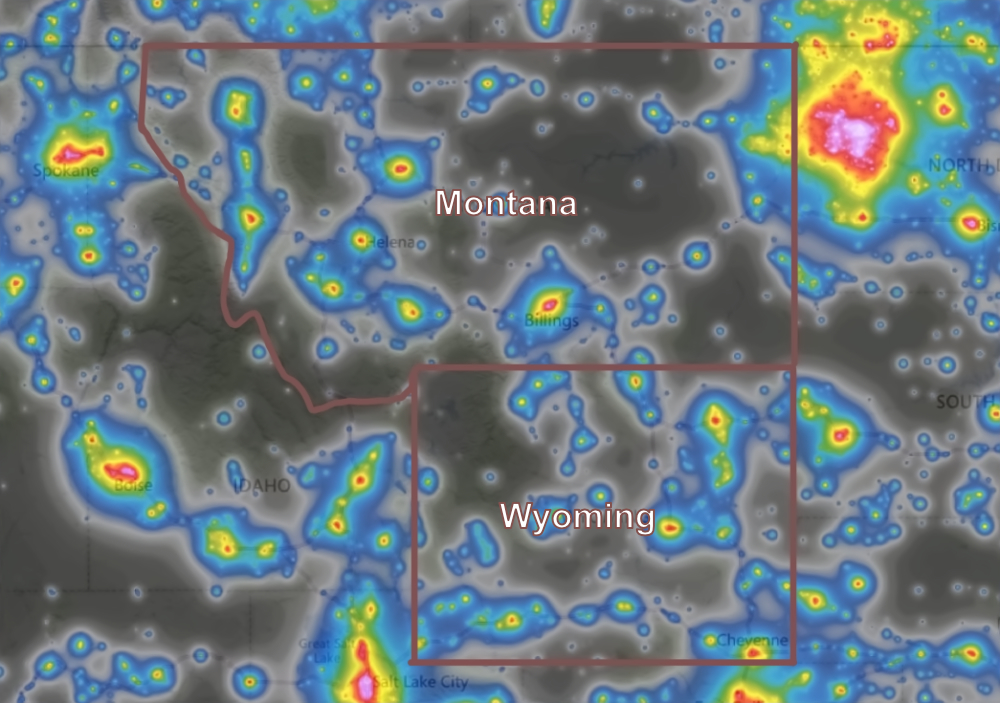
\includegraphics[width=1\textwidth]{figures/texted/Wyoming.jpg}
    \caption{Night-time Light Intensity of Wyoming} \label{fig:figure3}
\end{figure}
\subsubsection{A Rural Community: Nevada}

\subsubsection{A Suburban Community: California}
\begin{figure}[H]\centering
    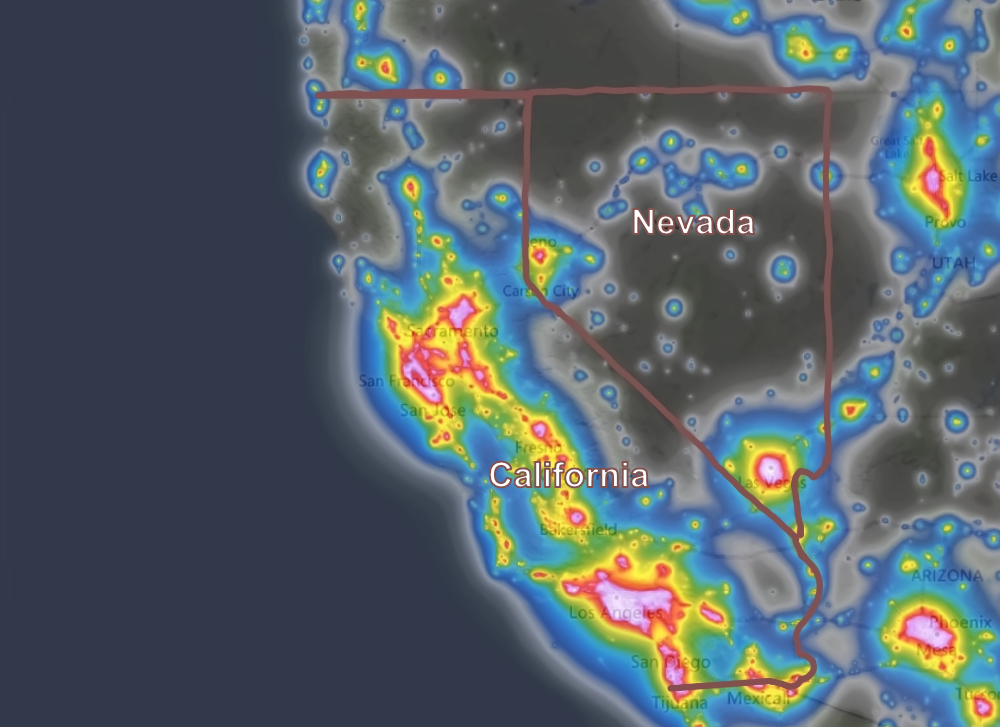
\includegraphics[width=1\textwidth]{figures/texted/Nevada.jpg}
    \caption{Night-time Light Intensity of California and Nevada} \label{fig:figure4}
\end{figure}
\subsubsection{An Urban Community: New York}
\begin{figure}[H]\centering
    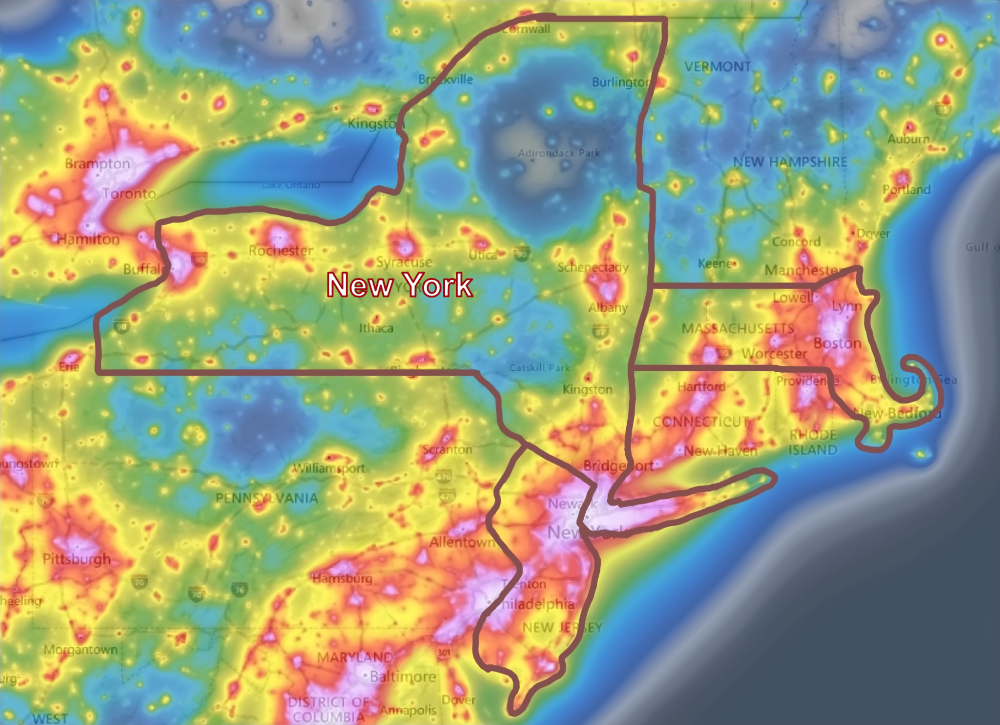
\includegraphics[width=1\textwidth]{figures/texted/New_York.jpg}
    \caption{Night-time Light Intensity of New York State} \label{fig:figure5}
\end{figure}
